\section{Material test - water purification}
In this study the capacity of different materials (concrete, zeolite, goethite,
ion exchange and activated carbon) to adsorb metal ions in polluted water over
time was investigated. The material were added in SpinChems rotating
bed reactors (RBR). The materials were sieved (300-700~$\mu$m) and washed in
deionized water before studied. The concentration of metal ions (copper and
zinc) was measured by the analytic methods FAAS and ICP-OES.

The spectro analytical method atomic absorption spectroscopy (AAS) determines
the concentration of metal ions by taken up the solution in a heated flame,
where the metal ions excites and absorb light that passes the flame specific
for the metal ion (Ford, M. A; Atomic absorption spectroscopy. Nature. 1979,
Vol.278, p.584)\todo{flytta}. The analytical technique inductively coupled plasma optical
emission spectroscopy (ICP-OES) is used for measuring metal ions. It produce
excited atoms and ions by using the inductively coupled plasma at wavelength
that is specific for the metal ion\todo{Källa}. The analytical methods has
different detection limits depending on machine and metal ions, but in general
ICP-OES can detect lower levels of metal ion concentration than FAAS. ICP-OES
can also analyze several metal ions at the same measurement while FAAS only
analyze one metal ion at a time.

To measure metal ion concentration 20~ml material was added to the
RBR S221 in the SpinChem reaction vessel V211 contained 200~ml polluted water
and rotated at 700~rpm during two time intervals. Before starting the stirrer
motor, a reference sample was taken and then samples were taken during a time
interval. In the first set, all materials were investigated separately and
samples were taken three times: 30~min, 60~min and 120~min. The experiment was
repeated for concrete, zeolites and goethite with time interval: 10~sec, 1~min,
3~min, 7~min, 15~min and 30~min. All samples were taken with a syringe and
filtered into falcon tubes. To each ml sample, 10~$\mu$l 7~M nitric acid was added
in the falcon tubes and sent to FAAS analysis.

After FAAS analyze, goethite was chosen for ICP-OES analyze to further
investigate its capacity to adsorb metal ions. 50~ml material was added to the
SpinChem RBR S331 in the reaction vessel V311 contained 1.2~l
polluted water and rotated at 700~rpm. Nine samples including the reference
sample were taken with a time interval: 0~min, 10~sec, 1~min, 3~min, 7~min, 15~min,
30~min, 1~h and 2~h. All samples were taken with a syringe and filtered
into falcon tubes. To each ml sample, 10~$\mu$l 7~M nitric acid was added in the
falcon tubes and analyzed with ICP-OES.

To examine how the material (concrete and goethite) affect pH during the
reaction 20~ml material was added to the RBR in the reaction vessel V211
contained 200~ml polluted water and rotated at 700~rpm. pH
was measured with litmus paper during a two hour period.

\subsection{Results}
The capacity of the different materials (concrete, zeolite, goethite, ion
exchange and activated carbon) to adsorb metal ions in polluted water over time
was analysed. The metal ions, zinc and copper, were measured with the analytic
methods FAAS and ICP-OES.

The FAAS analysis for the concentration of Zn$^{2+}$-ions showed that the
concentration of ions decreased for all materials after 30~minutes (figure
1\todo{fixa}). The same reference sample was used for all material. Goethite was the
material that decreased most after 120~min, while concrete was the material
with the lowest adsorption capacity. Between 30~min and 120~min, the
concentration of Zn$^{2+}$-ions increased with concrete as material. The FAAS
analysis for the concentration of Cu$^{2+}$-ions showed that the concentration of
Cu$^{2+}$-ions decreased for all materials except zeolites after 120~min (figure 2\todo{fixa}).
Between 60~min and 120~min, the concentration of Cu$^{2+}$-ions increased for
concrete.

\begin{figure}[H]
    \centering
    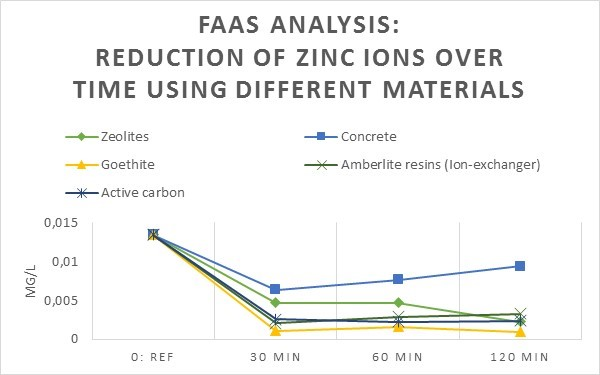
\includegraphics[width=0.7\textwidth]{image00}
    \caption{The concentrations of Zn$^{2+}$-ions in mg/l measured at four time
        points (0 min, 30 min, 60 min and 120 min) in five different materials
            (zeolites, goethite, active carbon, concrete and Amberlite resins)
            using the analytic method FAAS.}
\end{figure}


\begin{figure}[H]
    \centering
    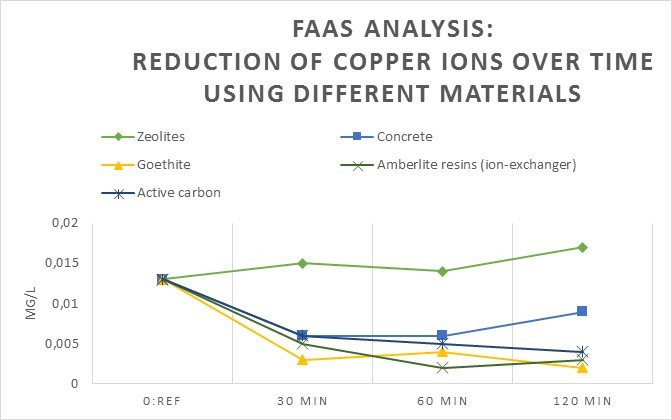
\includegraphics[width=0.7\textwidth]{image01}
    \caption{The concentrations of Cu$^{2+}$-ions in mg/l measured at four time
        points (0 min, 30 min, 60 min and 120 min) in five different materials
            (zeolites, goethite, active carbon, concrete and Amberlite resins)
            using FAAS analysis.}
\end{figure}

The experiment was repeated for zeolites, concrete and goethite but with
shorter time interval and more frequent sampling. The concentration of Zn$^{2+}$-ion
was analysed with FAAS. After 10 seconds the concentration of Zn$^{2+}$-ions had
increased for all materials (figure 3\todo{fixa}). After 30~min, goethite was the material
that had adsorb most Zn$^{2+}$-ions and with concrete as material, the concentration
of Zn$^{2+}$-ions started to increase after 7~min.

\begin{figure}[H]
    \centering
    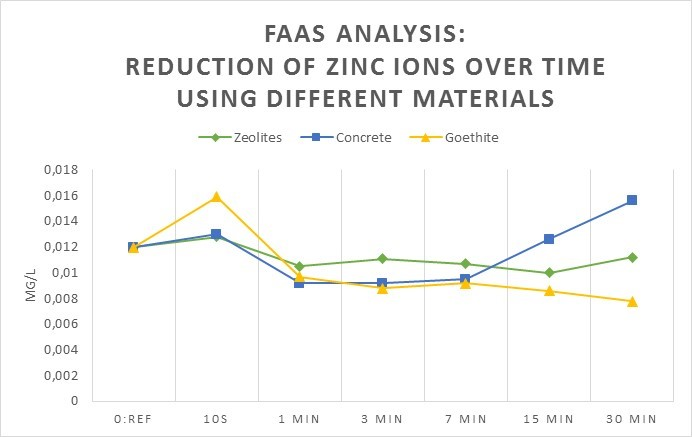
\includegraphics[width=0.7\textwidth]{image02}
    \caption{The concentrations of Zn$^{2+}$-ions in mg/l measured at seven time
        points (0 min, 10 s, 1 min, 3 min, 7 min, 15 min and 30 min) in three
            different materials (zeolites, concrete and goethite) using FAAS
            analysis.}
\end{figure}

The result for the ICP-OES analysis with goethite showed that the concentration
of Cu$^{2+}$-ions decreased until 15~min and between 15~min and 120~min the
concentration was stable at 0.02~mg/l (figure 4\todo{fixa}). The result for the
concentration of Zn$^{2+}$-ions with goethite displayed negative values but it seems
to decrease until 3~min and then flatten out (figure 5\todo{fixa}).

\begin{figure}[H]
    \centering
    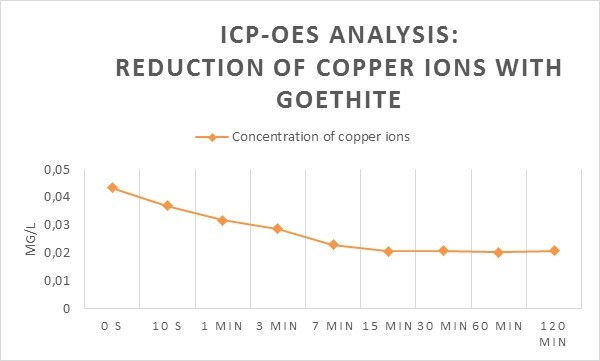
\includegraphics[width=0.7\textwidth]{image03}
    \caption{The concentration of Cu$^{2+}$-ions in mg/l measured at nine time
        points (0 s, 10 s, 1 min, 3 min, 7 min, 15 min, 30 min, 60 min and 120
                min) with goethite and analysed with ICP-OES.}
\end{figure}


\begin{figure}[H]
    \centering
    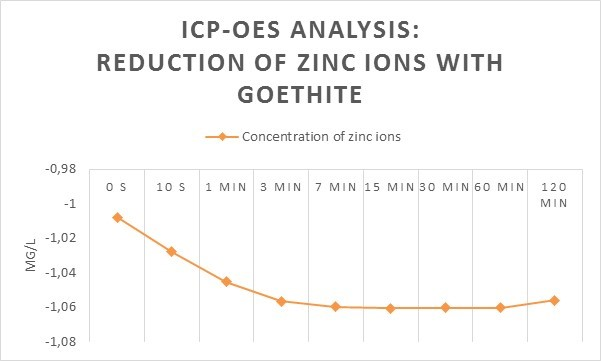
\includegraphics[width=0.7\textwidth]{image04}
    \caption{The concentration of Zn$^{2+}$-ions in mg/l measured at nine time
        points (0 s, 10 s, 1 min, 3 min, 7 min, 15 min, 30 min, 60 min and 120
                min) with goethite and analysed with ICP-OES.}
\end{figure}

The result for pH measurements of concrete and goethite in polluted water
containing metal ions showed unchanged pH at 5 for goethite during the whole
time interval (tab 1\todo{fixa}). For concrete, the pH raised from 5 to 10 the first 5~min
and then raised to 12 until 120~min.

\begin{table}[H]
\centering
\caption{pH measurements with litmus paper of concrete and goethite at eight
    time points (0 min, 5 min, 10 min, 15min, 30 min, 60 min, 90 min and 120
            min) in polluted water containing metal ions.}
\label{tab:ph}
\begin{tabular}{lllllllll}
minutes         & 0 & 5 & 10 & 15 & 30 & 60 & 90 & 120 \\
pH for concrete & 5 & 10 & 11 & 11 & 12 & 12 & 12 & 12 \\
pH for goethite & 5 & 5 & 5 & 5 & 5 & 5 & 5 & 5
\end{tabular}
\end{table}

\subsection{Discussion}
A part of this project was use SpinChem RBR and evaluate the
capacity of different materials to adsorb metal ions in solution over time. The
results from the FAAS analysis showed that all materials adsorb Zn$^{2+}$-ions after
120~min but had different capacities (fig 1\todo{fixa}). The concentration of Zn$^{2+}$-ions in
the solution decreased most the first 30~min and then the levels were quite
stable. This can be due to that the materials became saturated and was not able
to adsorb more Zn$^{2+}$-ions. The results also showed that concrete seemed to leak
out Zn$^{2+}$-ions back to the solution after 30~min. This might be because the bond
between Zn$^{2+}$-ions and concrete is weak and unstable or it favours other ions in
the solution. The results for Cu$^{2+}$-ions showed that all materials except
zeolites were able to adsorb first 30~min (fig 2). As for the materials to
adsorb Zn$^{2+}$-ions the result showed a similar pattern and after 30~min the
concentration of Cu$^{2+}$-ions were quite stable. This could be due to that the
materials became saturated and was not able to adsorb more Cu$^{2+}$-ions. It seems
like the zeolite is not able to adsorb Cu$^{2+}$-ions and might has greater affinity
for other ions.

Since the result for Zn$^{2+}$-ions showed a large decrease the first 30~min for all
material we chose to repeat the experiment with zeolite, concrete and goethite
during a shorter time interval and with more time points. The result was
unexpected because the concentration of Zn$^{2+}$-ions were quite unchanged during
the 30~min (fig 3\todo{fixa}). This could be due to that the standard that has to be
prepared for FAAS analysis was too high comparing to our samples and therefore
no conclusion can be made from this result.

After FAAS analysis we decided to continue the study with goethite since it had
the highest capacity to adsorb Zn$^{2+}$-ions and Cu$^{2+}$-ions (fig 1, 2, 3\todo{fixa}). We
repeated the experiment in larger scale (1.2~l) and chose to analyse with
ICP-OES. The result showed that the reduction of Cu$^{2+}$-ions in solution
decreased most first 15~min and then the concentration were quite stable at
0.02 (fig 4\todo{fixa}). Goethite seems to become saturated after 15~min and therefore not
able to adsorb more Cu$^{2+}$-ions. The result for the concentration of Zn$^{2+}$-ions in
solution showed negative values of the concentration but displayed a similar
pattern as for Cu$^{2+}$-ions (fig 5\todo{fixa}). Goethite seems to be able to adsorb Cu$^{2+}$-ions
the first 7~min and then become saturated. The negatively values can be due to
some error of measurement in ICP-OES machine.

The pH measurements for concrete and goethite gave different results. For
goethite, the pH level was stable around 5 during the whole time interval (tab 1\todo{fixa}).
This might be due to that the material bind to other ions or
release ions that does not affect the pH. The pH raised from 5 to 12 the whole
time range and the large increase of the pH could be that concrete leaked out
ions that affected the pH. The material could also bind hydrogen ions that
affect the pH.

In summary, goethite seems to have best capacity to adsorb Zn$^{2+}$-ions and
Cu$^{2+}$-ions comparing with the other materials and concrete seems to leak out the
metal ions after time. Since the concentration of metal ions was extremely low
in the solution, already in the beginning, the analysis methods seemed not to
be good enough as analytical tool for the study and in future a more sensitive
method should be used.

